% Search for all the places that say "PUT SOMETHING HERE".

\documentclass[11pt]{article}
\usepackage{amsmath,textcomp,amssymb,geometry,graphicx,enumerate,listings,color}

\def\Name{Derek Liu}  % Your name
\def\SID{3033954824}  % Your student ID number
\def\HWType{Lab}
\def\Homework{n} % Number of Homework
\def\Session{Fall 2020}
\graphicspath{ {./figures/} }

\title{EE C128--Fall 2020 --- \HWType\ \Homework Solutions}
\author{\Name, SID \SID}
\markboth{EE C128--\Session\ \HWType\ \Homework\ \Name}{EE C128--\Session\ \HWType\ \Homework\ \Name}
\pagestyle{myheadings}
\date{}

\newenvironment{qparts}{\begin{enumerate}[{(}a{)}]}{\end{enumerate}}
\def\endproofmark{$\Box$}
\newenvironment{proof}{\par{\bf Proof}:}{\endproofmark\smallskip}
%\renewcommand{\thesubsection}{\thesection.\alph{subsection}}
\newcommand{\fig}[3]{
\begin{figure*}[ht]
    \centering
    \includegraphics[scale=#1]{#2}
    \caption{#3}
\end{figure*}}

\textheight=9in
\textwidth=6.5in
\topmargin=-.75in
\oddsidemargin=0.25in
\evensidemargin=0.25in

\DeclareFixedFont{\ttb}{T1}{txtt}{bx}{n}{10} % for bold
\DeclareFixedFont{\ttm}{T1}{txtt}{m}{n}{10}  % for normal
\definecolor{deepblue}{rgb}{0,0,0.5}
\definecolor{deepred}{rgb}{0.6,0,0}
\definecolor{deepgreen}{rgb}{0,0.5,0}

\newcommand{\lstsetmatlab}{
\lstset{
language=MATLAB,
basicstyle=\ttfamily\small,
commentstyle=\ttfamily\small\color{deepgreen}, 
otherkeywords={self,None},             % Add keywords here
keywordstyle=\ttb\color{deepblue},
emph={MyClass,__init__},          % Custom highlighting
emphstyle=\ttb\color{deepred},    % Custom highlighting style
stringstyle=\color{deepred},
frame=tb,                         % Any extra options here
breaklines=true,
breakatwhitespace=true,
postbreak=\mbox{\textcolor{red}{$\hookrightarrow$}\space},
showstringspaces=false,            % 
morestring=[b]"
%moredelim=[s][\color{deepred}]{"""}{"""}
%morecomment=[s]{"""}{"""}\color{deepred}
}}
\newcommand{\lstsetpython}{
\lstset{
language=Python,
basicstyle=\ttfamily\small,
commentstyle=\ttfamily\small\color{deepgreen}, 
otherkeywords={self,None},             % Add keywords here
keywordstyle=\ttb\color{deepblue},
emph={MyClass,__init__},          % Custom highlighting
emphstyle=\ttb\color{deepred},    % Custom highlighting style
stringstyle=\color{deepred},
frame=tb,                         % Any extra options here
breaklines=true,
breakatwhitespace=true,
postbreak=\mbox{\textcolor{red}{$\hookrightarrow$}\space},
showstringspaces=false,            % 
morestring=[b]"
%moredelim=[s][\color{deepred}]{"""}{"""}
%morecomment=[s]{"""}{"""}\color{deepred}
}}

\begin{document}

\setcounter{section}{3}
\section{}
\setcounter{subsection}{2}
\subsection{}
\fig{0.54}{q43_alt.png}{Altitude plot.}
\fig{0.54}{q43_vel.png}{Velocity plot.}
\fig{0.54}{q43_rot.png}{Rotation angle plot.}

%TODO: fill out
\newpage\clearpage
\section{}

\subsection{System Identification}
We chose the frequencies 0.5, 0.75, 1.0, 2.0, and 4.0 rad/s. 
\fig{0.54}{q51_time0.5.png}{$\omega = 0.5$ rad/s}
\fig{0.54}{q51_time0.75.png}{$\omega = 0.75$ rad/s}
\fig{0.54}{q51_time1.0.png}{$\omega = 1.0$ rad/s}
\fig{0.54}{q51_time2.0.png}{$\omega = 2.0$ rad/s}
\fig{0.54}{q51_time4.0.png}{$\omega = 4.0$ rad/s}

\fig{0.84}{q51_ft_0.5.png}{FFT for $\omega = 0.5$ rad/s}
\fig{0.84}{q51_ft_0.75.png}{FFT for $\omega = 0.75$ rad/s}
\fig{0.84}{q51_ft_1.0.png}{FFT for $\omega = 1.0$ rad/s}
\fig{0.84}{q51_ft_2.0.png}{FFT for $\omega = 2.0$ rad/s}
\fig{0.84}{q51_ft_4.0.png}{FFT for $\omega = 4.0$ rad/s}

\newpage \clearpage
\fig{0.84}{q51_bode.png}{Bode plot derived from gains and phases. See code for how it was generated.
There are [TODO] poles and [TODO] zeros, and there exists a delay in the system. 
}

Code for plotting and calcuation:
\lstsetmatlab
\lstinputlisting[]{code/q51.m}

\newpage \clearpage
\subsection{Proportional control}

We use $k_P = 3$ for our proportional controller. The gain is [TODO] and the phase margin is [TODO], and we got this value from 
the estimation and some tuning.

Here's the code:
\lstsetpython
\begin{lstlisting}
# Controller Variables
kp = 3

# Control stores
integratedError = 0.0
errorStore = 0.0

# Useful Reference Signal Variables
period = 20
amplitude = 180

##### ... skip starter code ... #####

# Compute Reference Signal (Triangle wave)
reference = (2 * amplitude) / np.pi * np.arcsin(np.sin(2*np.pi * ptime / period))

# Compute Error and Control Input
error = reference - yaw
control_YA = kp * error
\end{lstlisting}

\begin{figure}
    \centering 
    \centerline{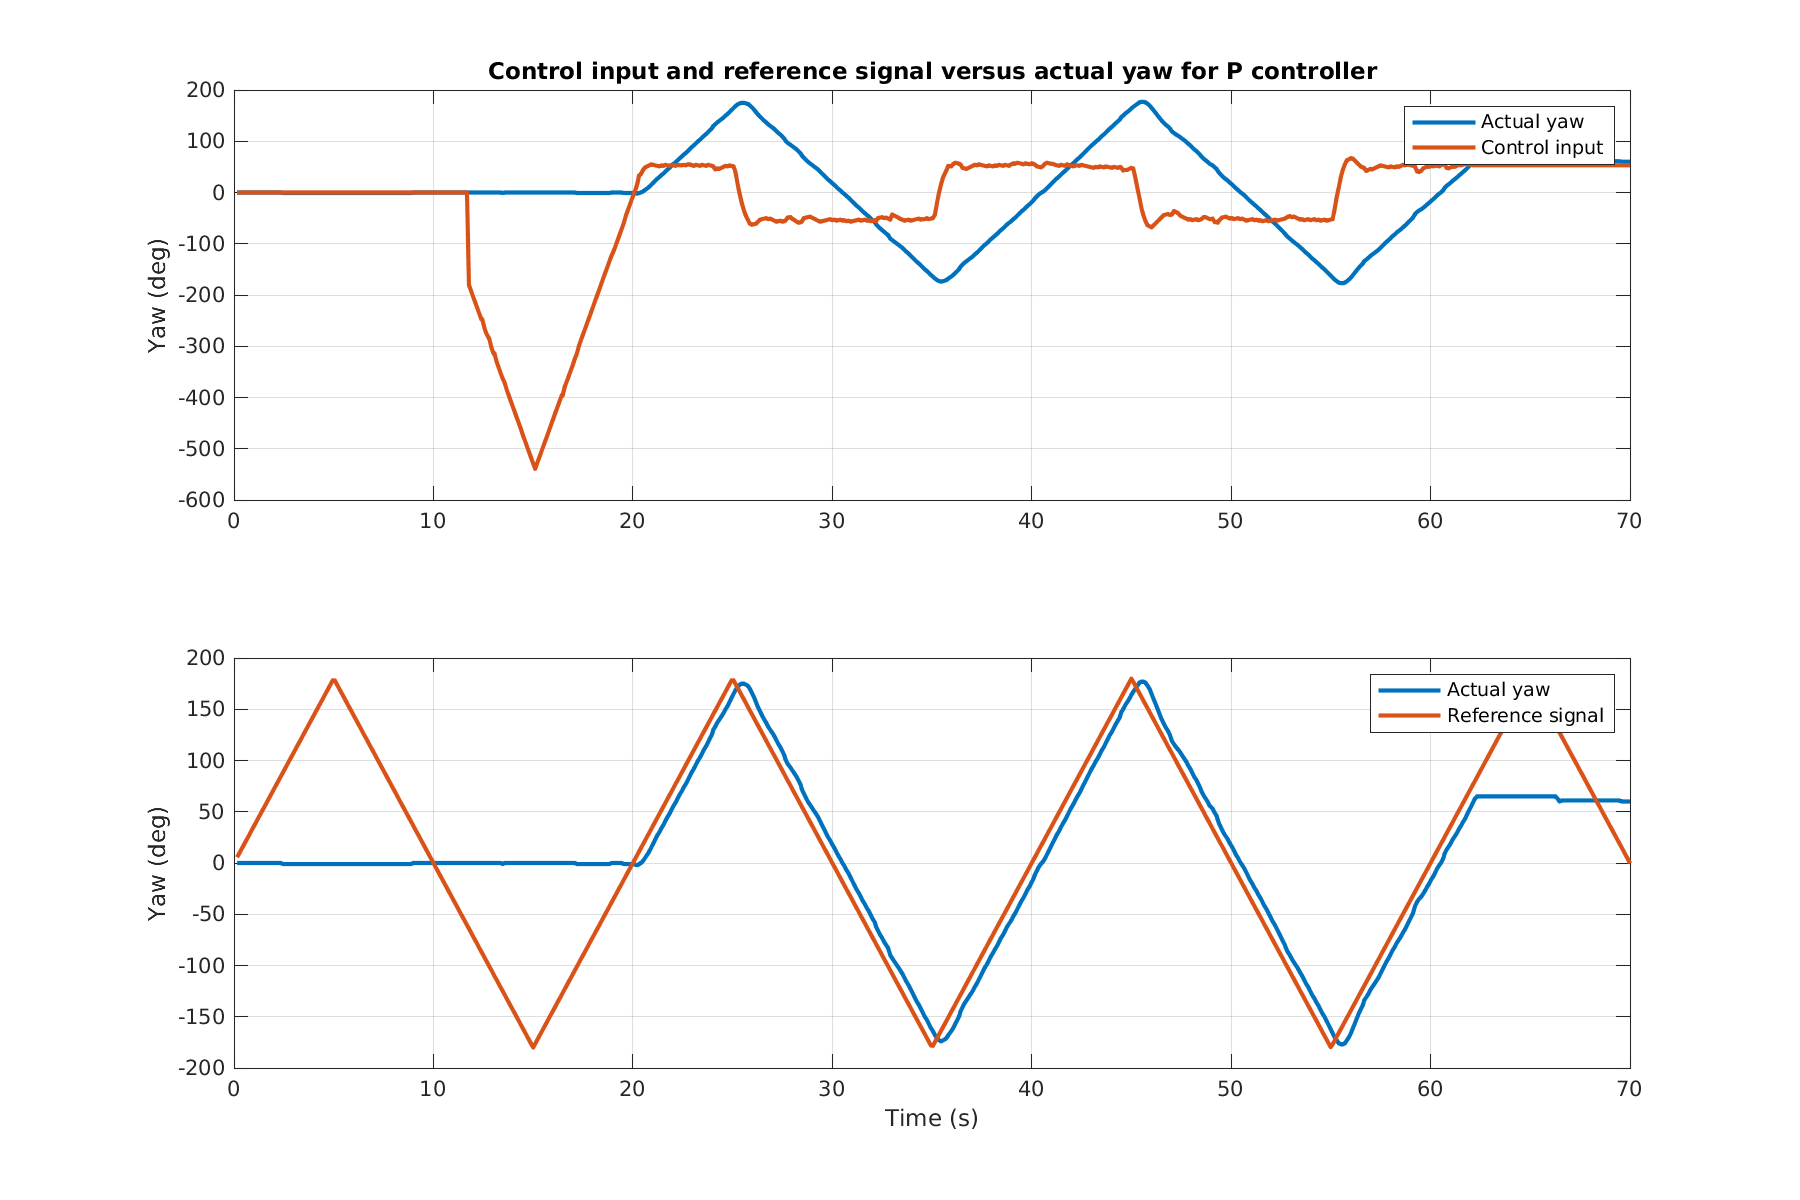
\includegraphics[scale=0.7]{q52.png}}
    \caption{Here's the plot. It actually tracks pretty well, although there is a small steady state error. }
\end{figure}

\newpage \clearpage
Here's plotting code:
\lstsetmatlab
\lstinputlisting[]{code/q52.m}

\subsection{Better Triangular Wave Tracking}
\subsubsection{Designing a controller}
We used a PI controller with $k_I = 0.5$ and an anti-windup decay term of $0.7$. 
Here's the code:
\lstsetpython
\begin{lstlisting}
# Controller Variables
kp = 3.0
ki = 0.05 
kw = 0.7 # decay term to avoid integral windup

###### skip starter code ######
# Compute Reference Signal (Triangle wave)
reference = (2 * amplitude) / np.pi * np.arcsin(np.sin(2*np.pi * ptime / period))

# Compute Error and Control Input
error = reference - yaw
integratedError = kw * integratedError + (ptime - lastTime) * error
control_YA = kp * error + ki * integratedError
\end{lstlisting}

\begin{figure}[ht]
    \centering 
    \centerline{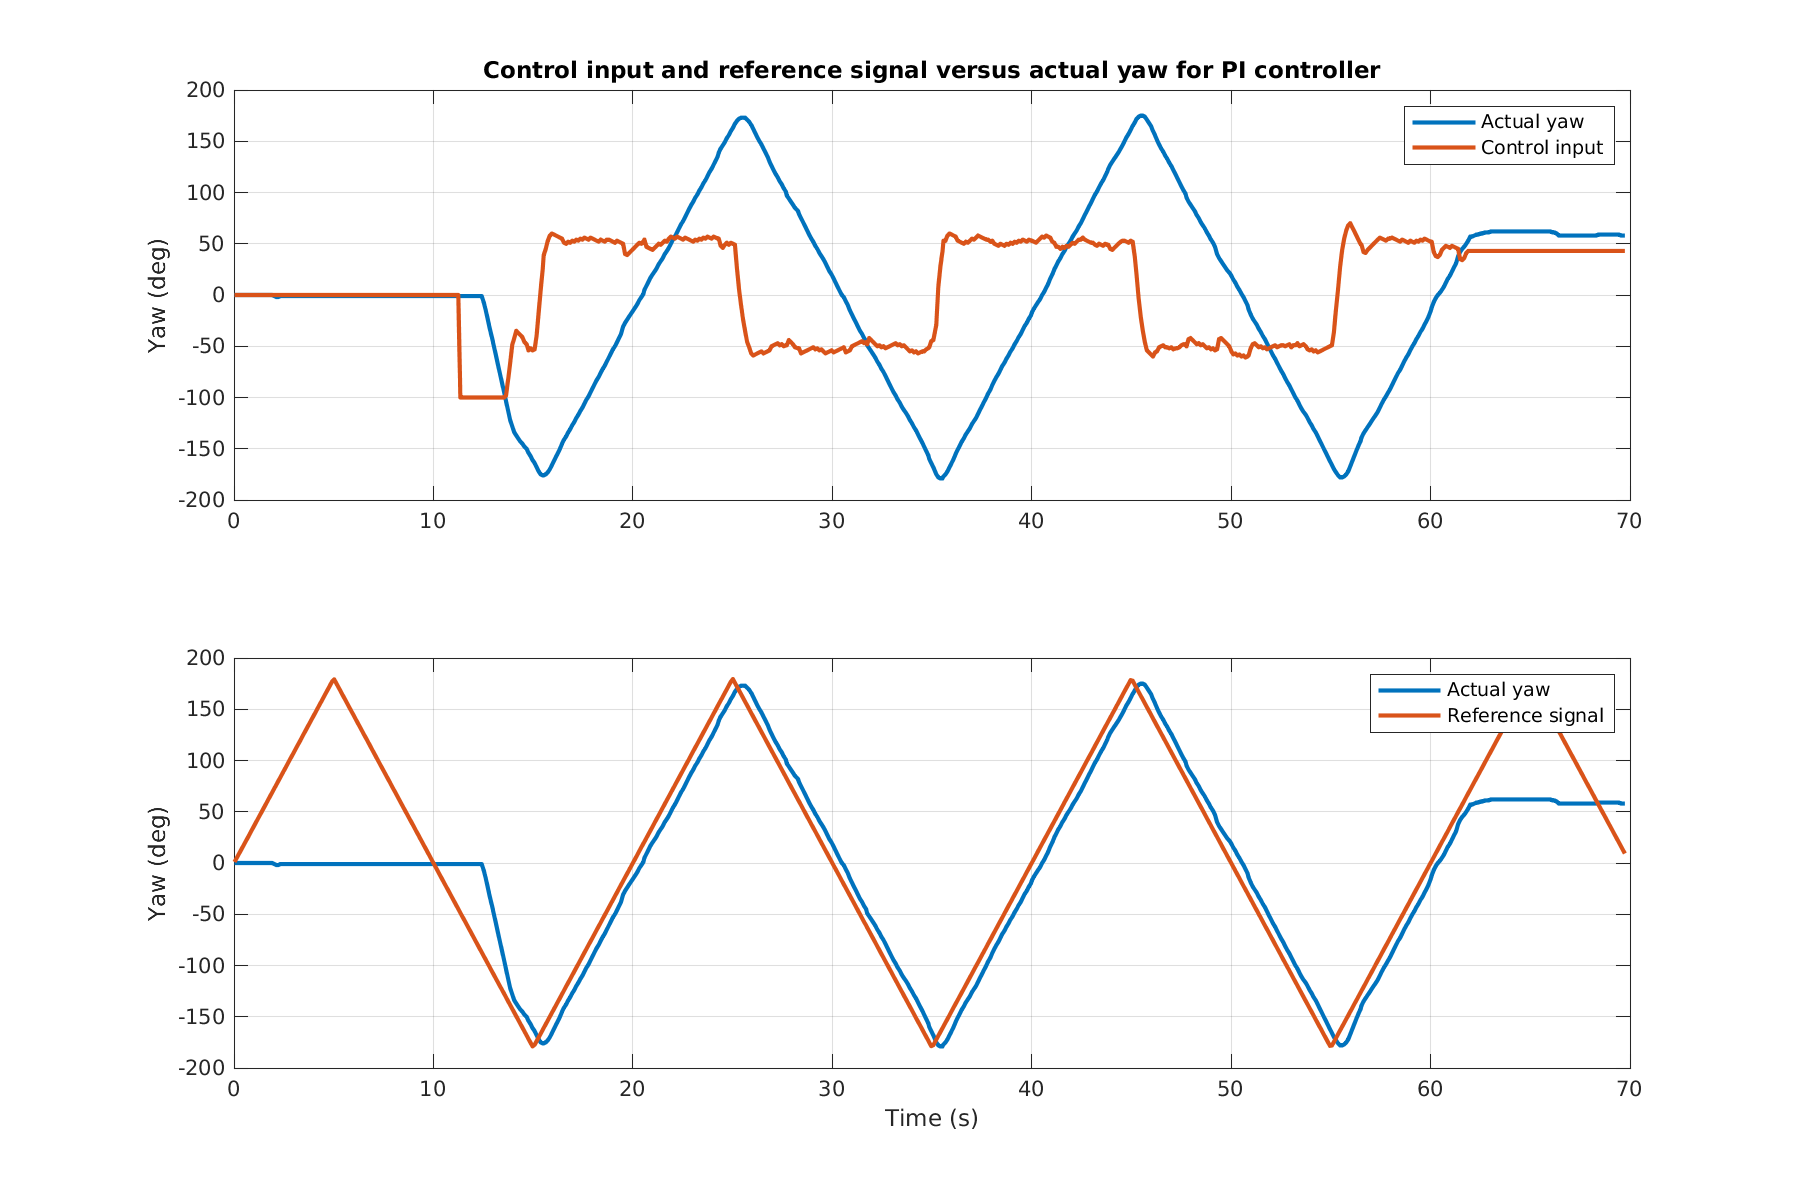
\includegraphics[scale=0.7]{q531.png}}
    \caption{Here's the plot. It still tracks well, but we were unable to remove the SSE entirely. }
\end{figure}

\newpage \clearpage

\subsubsection{Comparison to DJI's controller}
\begin{figure}[ht]
    \centering 
    \centerline{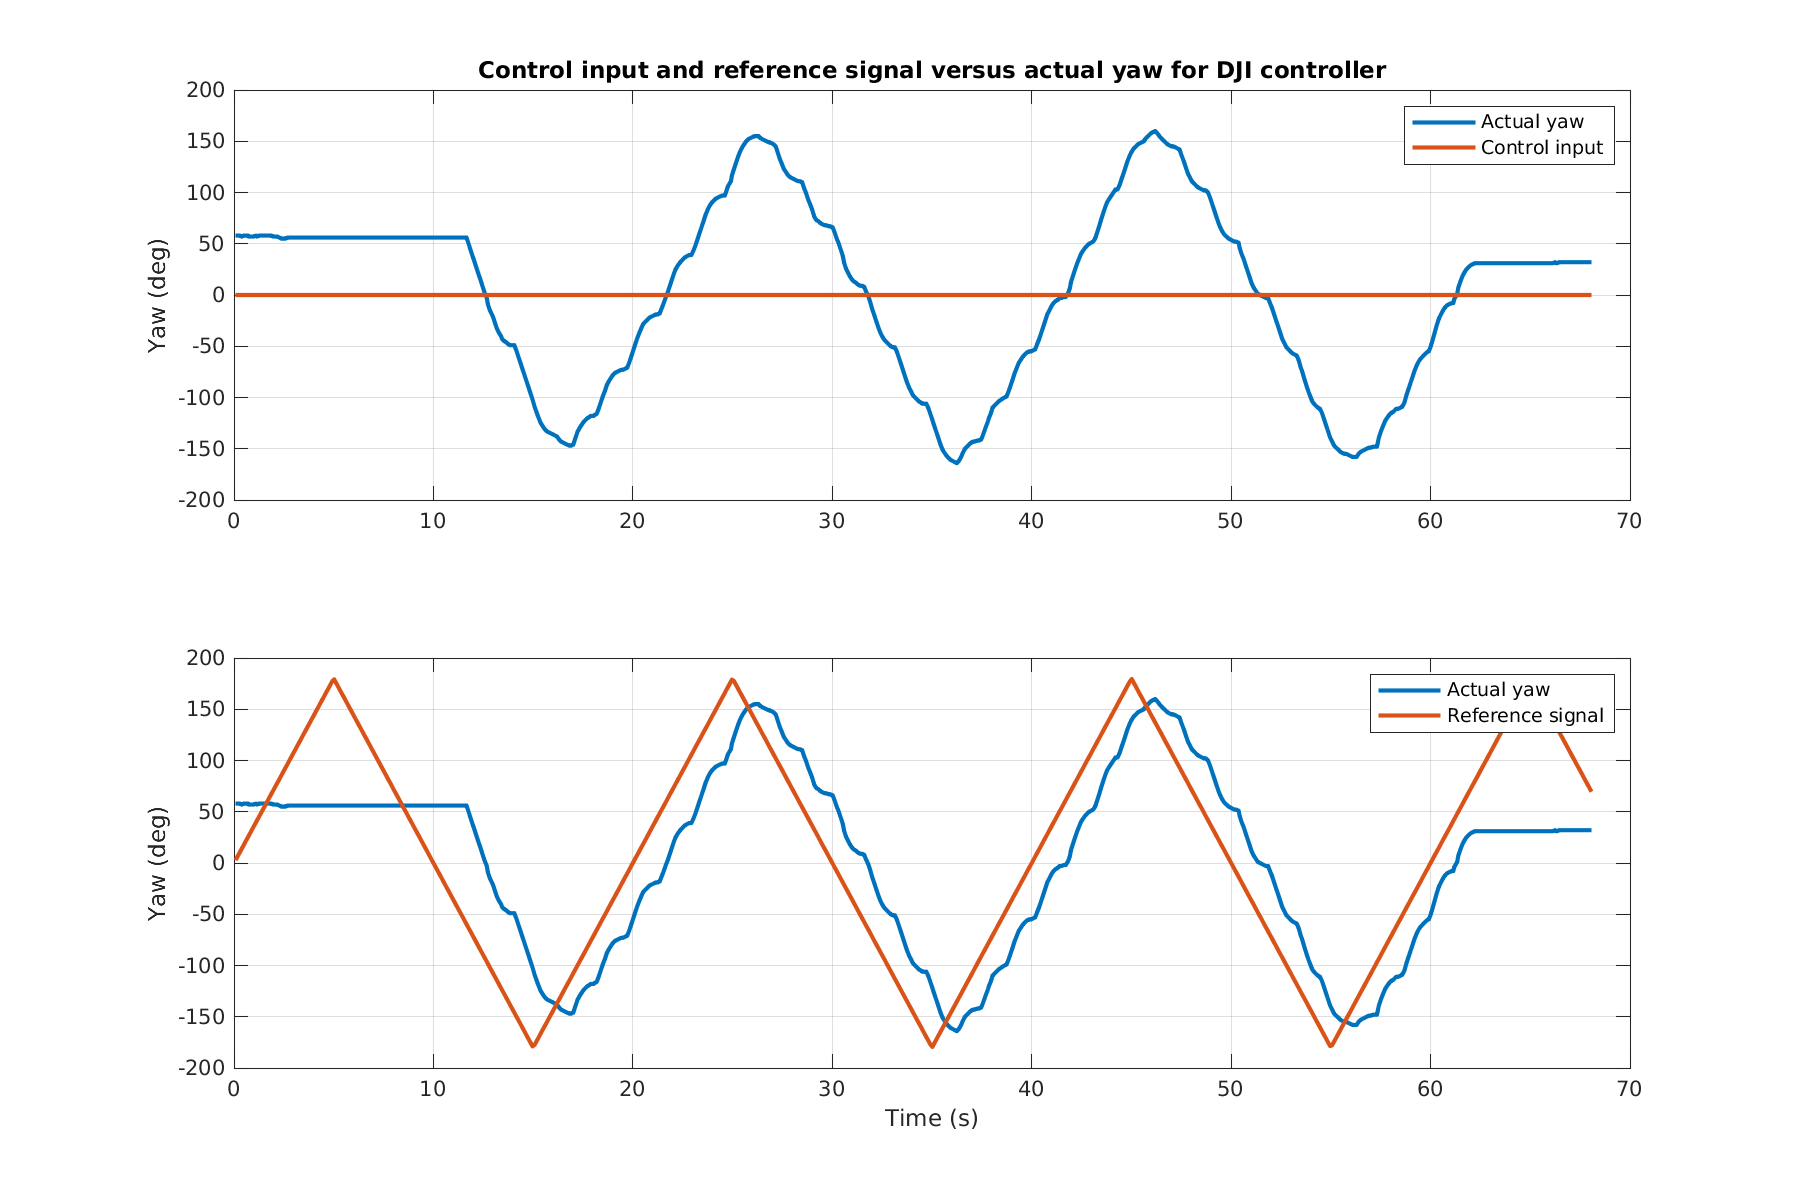
\includegraphics[scale=0.65]{q532.png}}
    \caption{Here's the plot. In DJI's defense, it seems rather dubious that the commands used to 
    attempt to follow the function were intended to be used for this sort of thing, as it seems to 
    be constantly updating a yaw position setpoint every 10 Hz instead of being fully smooth.}
\end{figure}

\newpage \clearpage

\subsection{Lab 5a comparisons}
%TODO: actually do
\begin{figure}[ht]
    \centering

    % Uncomment the line below after running q54.m to generate figures/q54.png
    %TODO: replace this image placeholder with the actual q54.png
    %\centerline{\includegraphics[scale=0.65]{q54.png}}
    \caption{Our system was not able to track as well, given the disturbances...}
\end{figure}
\end{document}
